\chapter{Refinement of the INTERLACE Business Logic Specification}
\label{ch:UpdateBLS}

\vspace{-1cm}
\begin{center}
Paolo Dini, Luca Carboni, Giuseppe Littera, and Chrystopher Nehaniv
\end{center}

\section{Context}
The business logic specification provided in Deliverable D2.1 \cite{INTERLACE_D21} concerns user-initiated transactions. Although this is a subset of all possible operations (initiated by the users or by the System) that a mutual credit system platform must support, it is a viable starting point for testing an initial executable CoreASIM model. D2.1 did not provide all the details of the transaction request operations, it left their specification at a fairly abstract level. This chapter provides the next step in the iterative refinement of the specification in the form of a detailed description of the Permissioning workflow, whose implementation as part of the CoreASIM model is then described in Chapter \ref{ch:CoreAsimImplementation}.

The description of the Permissioning iterative refinement relies mainly on graphical depictions of the variables and functions involved. As this reflects the process that was used to build a shared understanding within the INTERLACE team itself, it is hoped that it will also make it easier for newcomers to the INTERLACE open source community to understand the implementation.

\section{Overview}
Figure \ref{transactabilitywkflow} shows the high-level view of the process.

\begin{figure}[htbp]
\centering
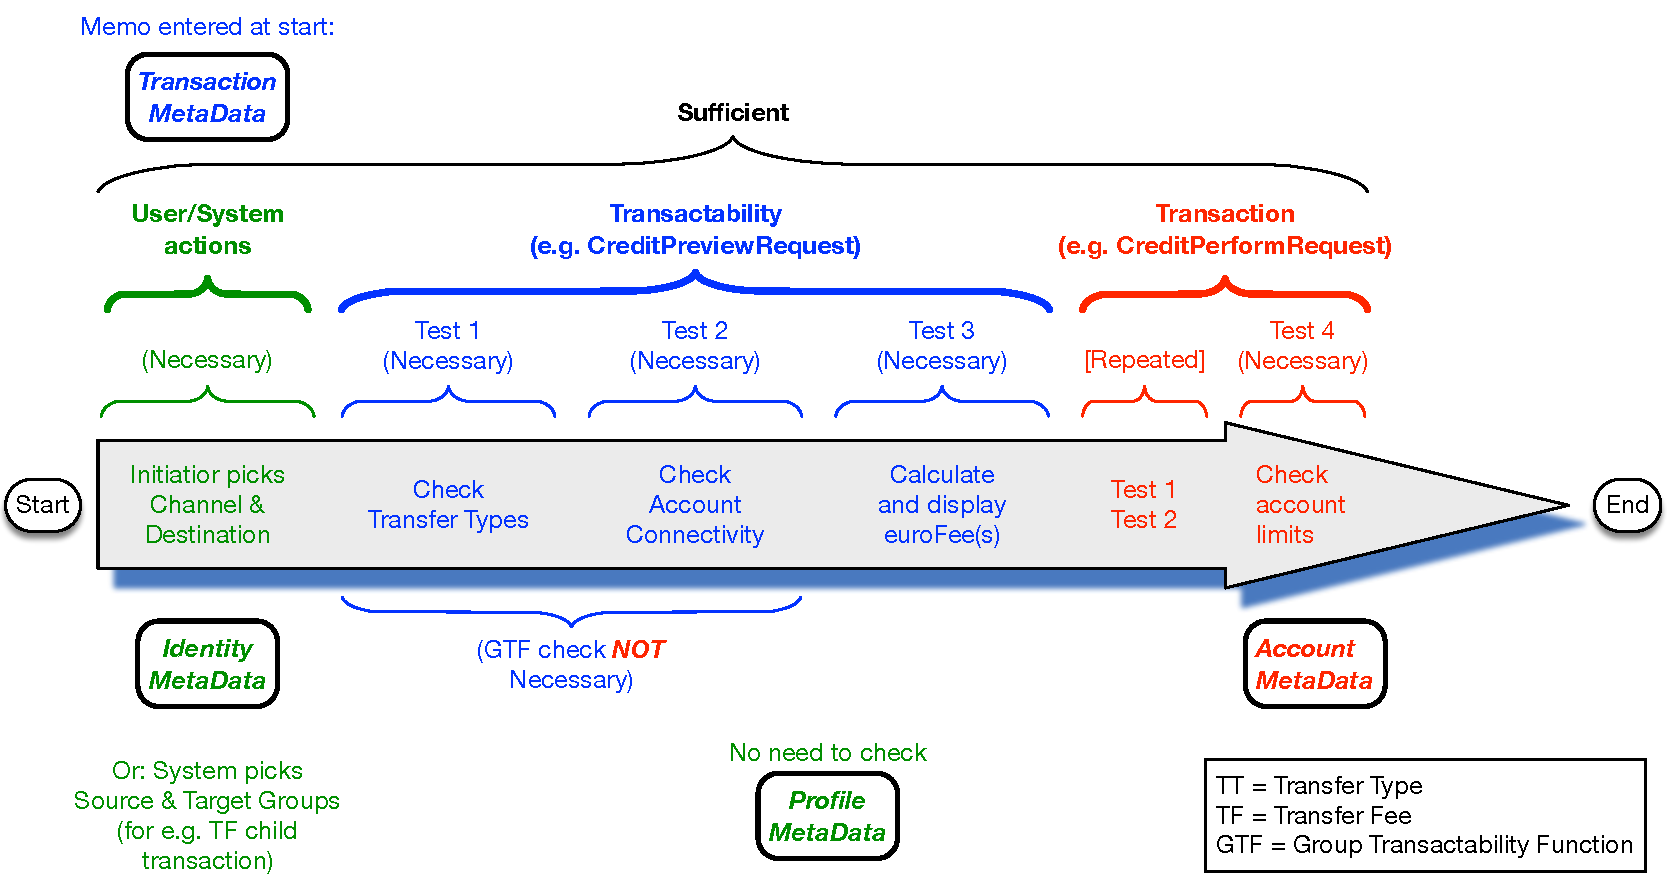
\includegraphics[width=16cm]{Figures/Transactability_Workflow}
\caption{\small\textbf{High-level workflow of the Permissioning process for user- or system-initiated transactions}}
\label{transactabilitywkflow}
\end{figure}






